
\documentclass{article}

\usepackage{amssymb}
\usepackage{amsmath}
\usepackage{pgfplots}
\usepackage{tikz}
\usepackage[top=0.9in, bottom=0.9in, left=1.5in, right=1.5in]{geometry}
\usepackage{xcolor}
\usepackage{xparse,mathtools}



\title{ECE421 Problem Set 3}
\author{Micol Altomare}
\date{October 11, 2023} 

\begin{document}

\maketitle


\section{SVM w. Hard Margin}



\subsection{}
(graph template, should label points for easy reference)

\begin{figure}[ht]
  \centering
  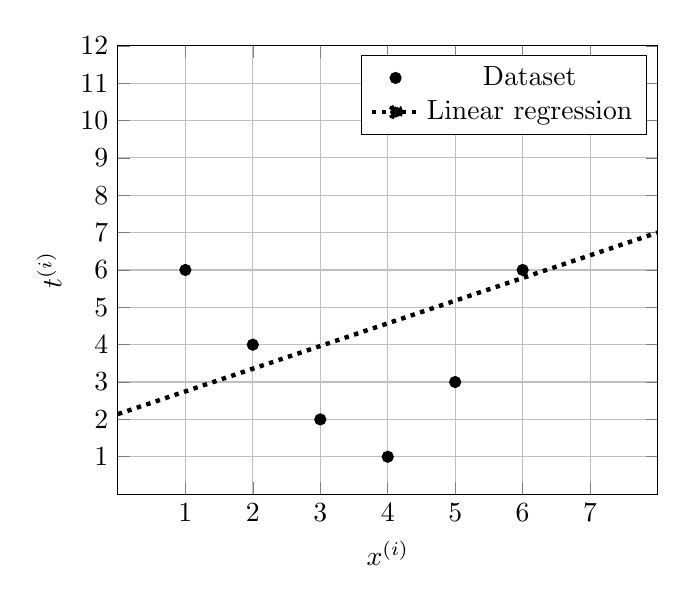
\begin{tikzpicture}
    \begin{axis}[
      xlabel={$x^{(i)}$},
      ylabel={$t^{(i)}$},
      xmin=0, xmax=8, 
      ymin=0, ymax=12,
      xtick={1,2,3,4,5,6,7},
      ytick={1,2,3,4,5,6,7,8,9,10,11,12},
      grid=both,
      mark=*,
      ]
      
      \addplot[only marks] table {
        1 6
        2 4
        3 2
        4 1
        5 3
        6 6
        7 10
      };
      \addlegendentry{Dataset}
	% question 1.5
      \addplot [dotted, domain=0:8, samples=2, ultra thick] {0.607142857*x + 2.142857143};
      \addlegendentry{Linear regression} //// mark=*????
    \end{axis}
  \end{tikzpicture}
  \caption{Scatter plot of $x^{(i)}$ vs. $t^{(i)}$}
\end{figure}
%%%%%%%%%%%%%%%%%%%%%%%%%%%%%%%%%%%%%%%%%%%%%%%%%%%%
%%%%%%%%%%%%%%%%%%%%%%%%%%%%%%%%%%%%%%%%%%%%%%%%%%%%
%%%%%%%%%%%%%%%%%%%%%%%%%%%%%%%%%%%%%%%%%%%%%%%%%%%%


\section{Binary linear classification vs. SVM}

\end{document}